\subsubsection{Latency \& Throughput}

Charts on Figures \ref{fig:persistent_app_latency}, \ref{fig:ephemeral_app_latency}, \ref{fig:persistent_app_throughput}, and \ref{fig:ephemeral_app_throughput} represent the \gls{p90} of Latency and Throughput of all 10000 requests made by the persistent and ephemeral clients during the experiments.

\subsubsection*{\gls{http}/1 and \gls{http}/2}

Local \gls{http}/1 experiment had the best results overall, with lowest latency and highest throughput. Local \gls{http}/2 was also at the top, only losing to \gls{http}/1 due to the extra features it implements overhead. For instance, \gls{http}/2 always compresses its requests/responses headers, but in these experiments there was close to nothing in the headers. Consequently, \gls{http}/2 spent some time dealing with compression, while \gls{http}/1 simply sent the request with headers in plain text. This pattern continues throughout Single-\gls{az} and Multi-\gls{az} experiments.

\subsubsection*{\gls{tls} Impact}

Both \gls{http}/1 and \gls{http}/2 maintained the previous observed pattern when using \gls{tls}. However, latency and throughput got worse due to \gls{tls}’ data encryption and \gls{tls} handshake requirements. The latter is better observed in the persistent experiments, while the former is the main reason for the further difference between protocols during ephemeral experiments.

\subsubsection*{\gls{http}/2+\gls{tls} and \gls{http}/3}

\gls{http}/3 starts with similar results to \gls{http}/2+\gls{tls}, but starting from the 32KiB payload it starts widening the difference between them both. As payload increases, QUIC only gets worse, further demonstrating it performs poorly on a reliable network when compared with \gls{http}/2+\gls{tls}. This is similar to the comparison between QUIC and \gls{tcp}+\gls{tls} protocols, since it appears they are the deciding factor when it comes to performance between \gls{http}/2 and \gls{http}/3.

\subsubsection*{QUIC's Handshake Efficiency}

Although HTTP/3 did not perform as well as HTTP/2+TLS, it managed to maintain the same behaviour as transport-layer experiments, since it was less impacted by ephemeral clients.

During the Multi-AZ scenario, while HTTP/2+TLS’ throughput went from 1600 Mb/s with persistent clients to 536 Mb/s with ephemeral clients, equivalent to a decrease of 66.5\%, HTTP/3’s throughput went from 425 Mb/s to 224 Mb/s, equivalent to a decrease of 47\% (Figures \ref{fig:persistent_app_throughput} and \ref{fig:ephemeral_app_throughput}). This demonstrates the impact of QUIC’s handshake since it only needs 1-\gls{rtt} with unknown servers, while TCP+TLS’ handshake requires, in general, 3-\gls{rtt}s.

\clearpage

\begin{figure}[h!]
    \centering
    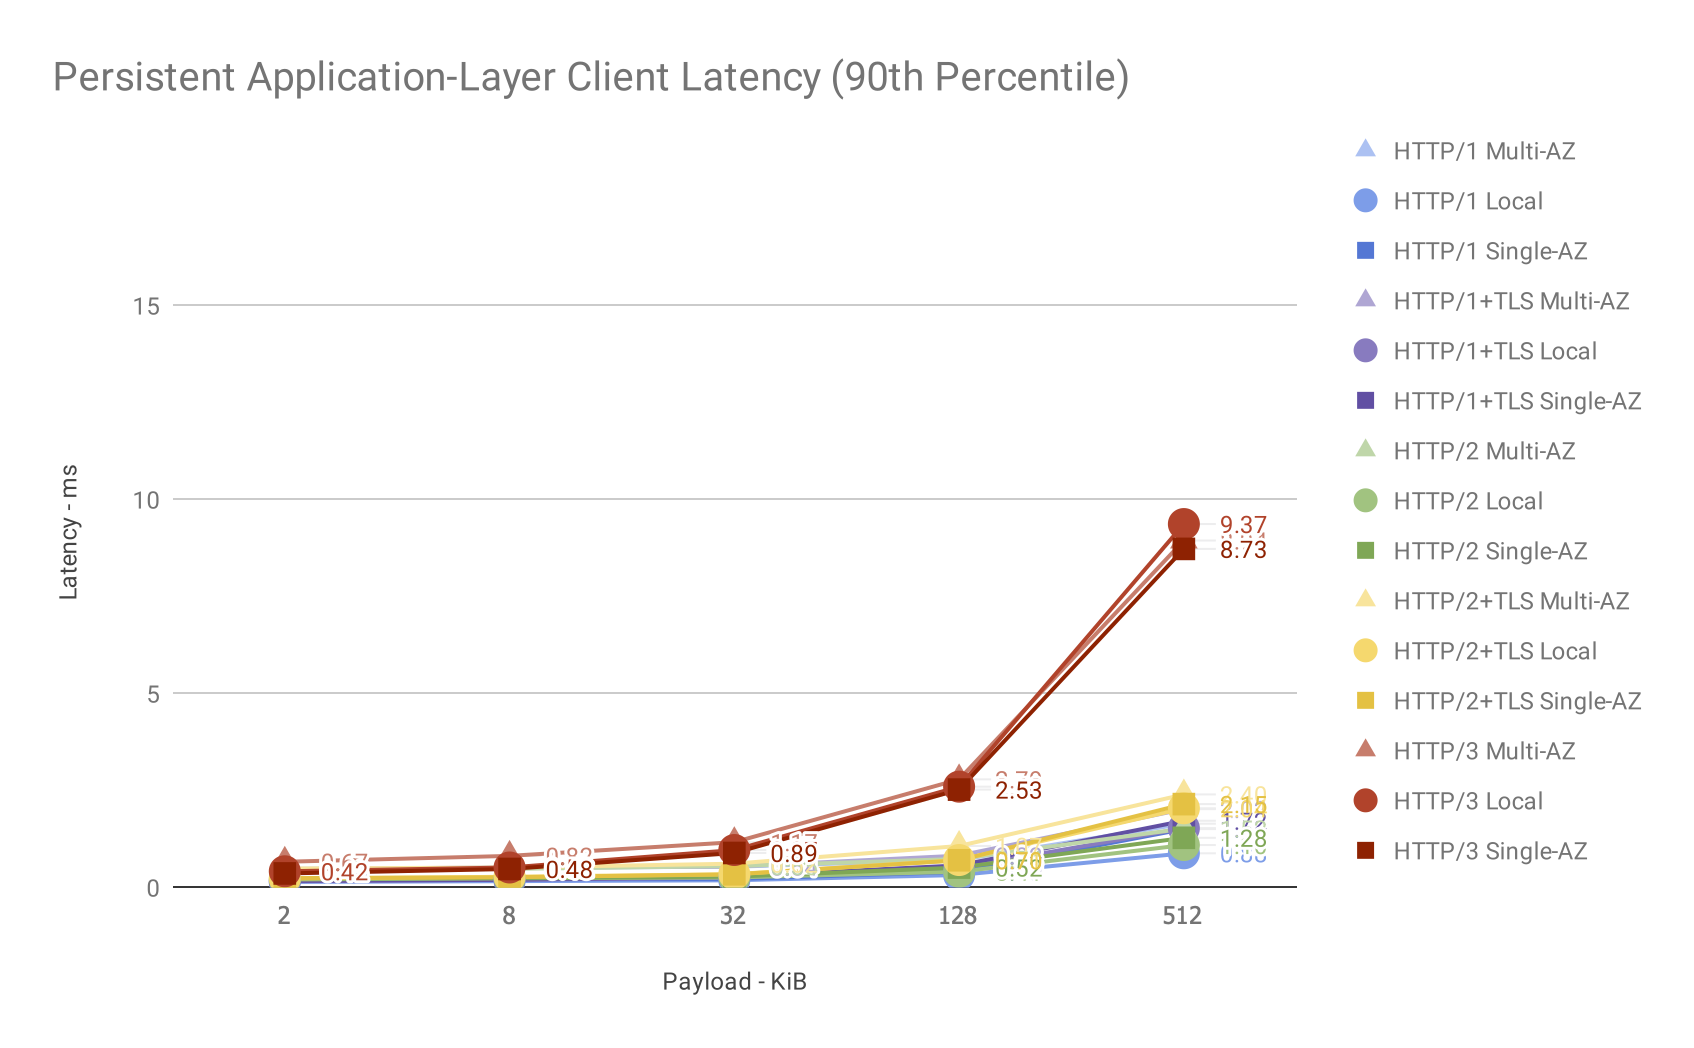
\includegraphics[width=\linewidth]{figures/charts/Persistent Application-Layer Client Latency (90th Percentile).png}
    \caption{Persistent Application-Layer Client Latency (90th Percentile)}
    \label{fig:persistent_app_latency}
\end{figure}
\begin{figure}[h!]
    \centering
    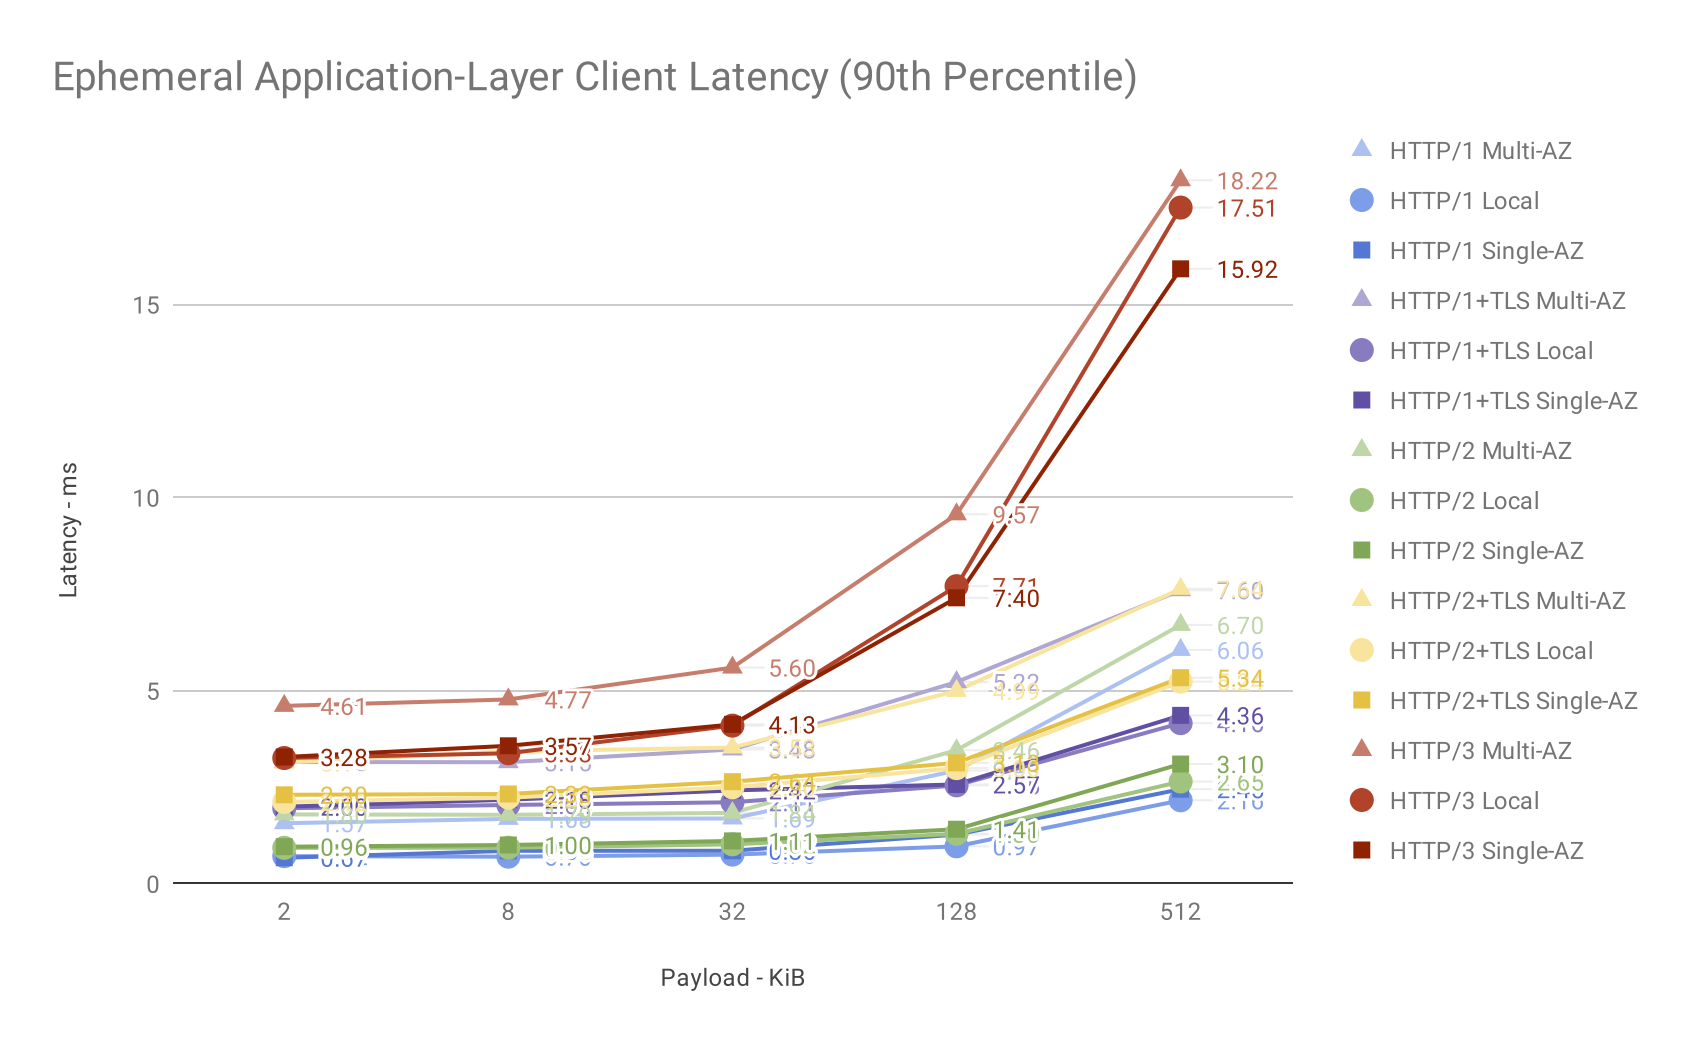
\includegraphics[width=\linewidth]{figures/charts/Ephemeral Application-Layer Client Latency (90th Percentile).png}
    \caption{Ephemeral Application-Layer Client Latency (90th Percentile)}
    \label{fig:ephemeral_app_latency}
\end{figure}

\clearpage

\begin{figure}[h!]
    \centering
    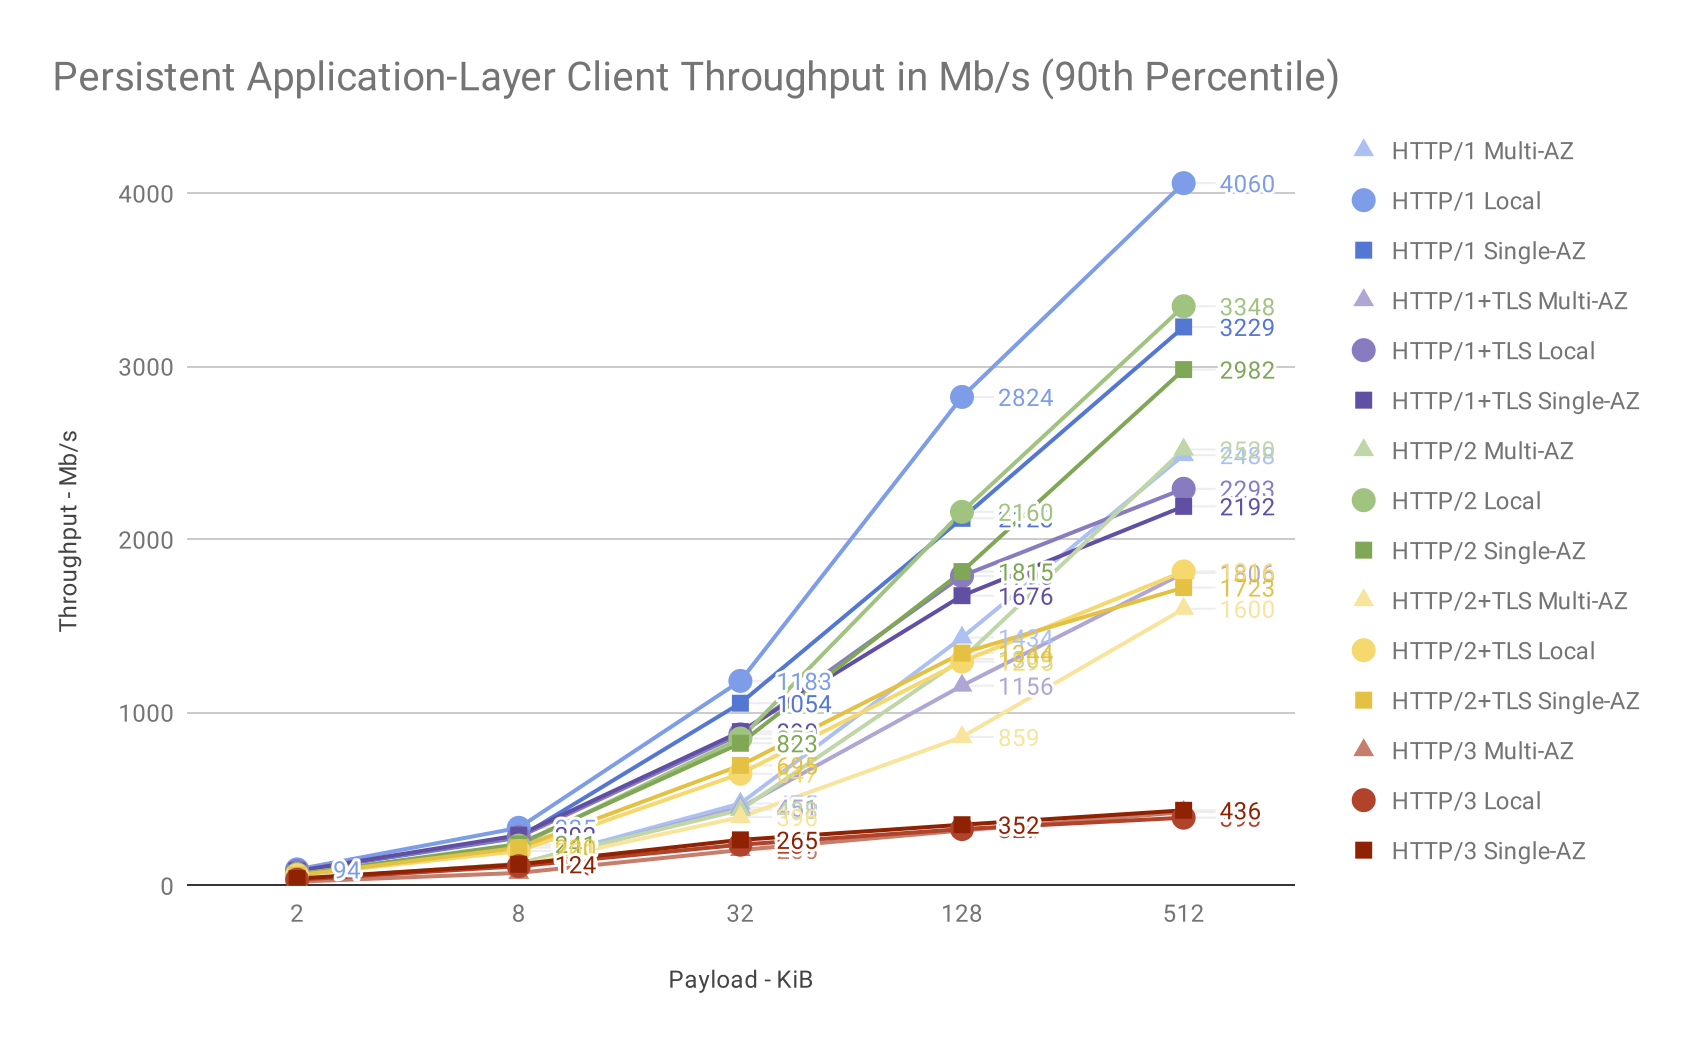
\includegraphics[width=\linewidth]{figures/charts/Persistent Application-Layer Client Throughput in Mb_s (90th Percentile).png}
    \caption{Persistent Application-Layer Client Throughput in Mb/s (90th Percentile)}
    \label{fig:persistent_app_throughput}
\end{figure}
\begin{figure}[h!]
    \centering
    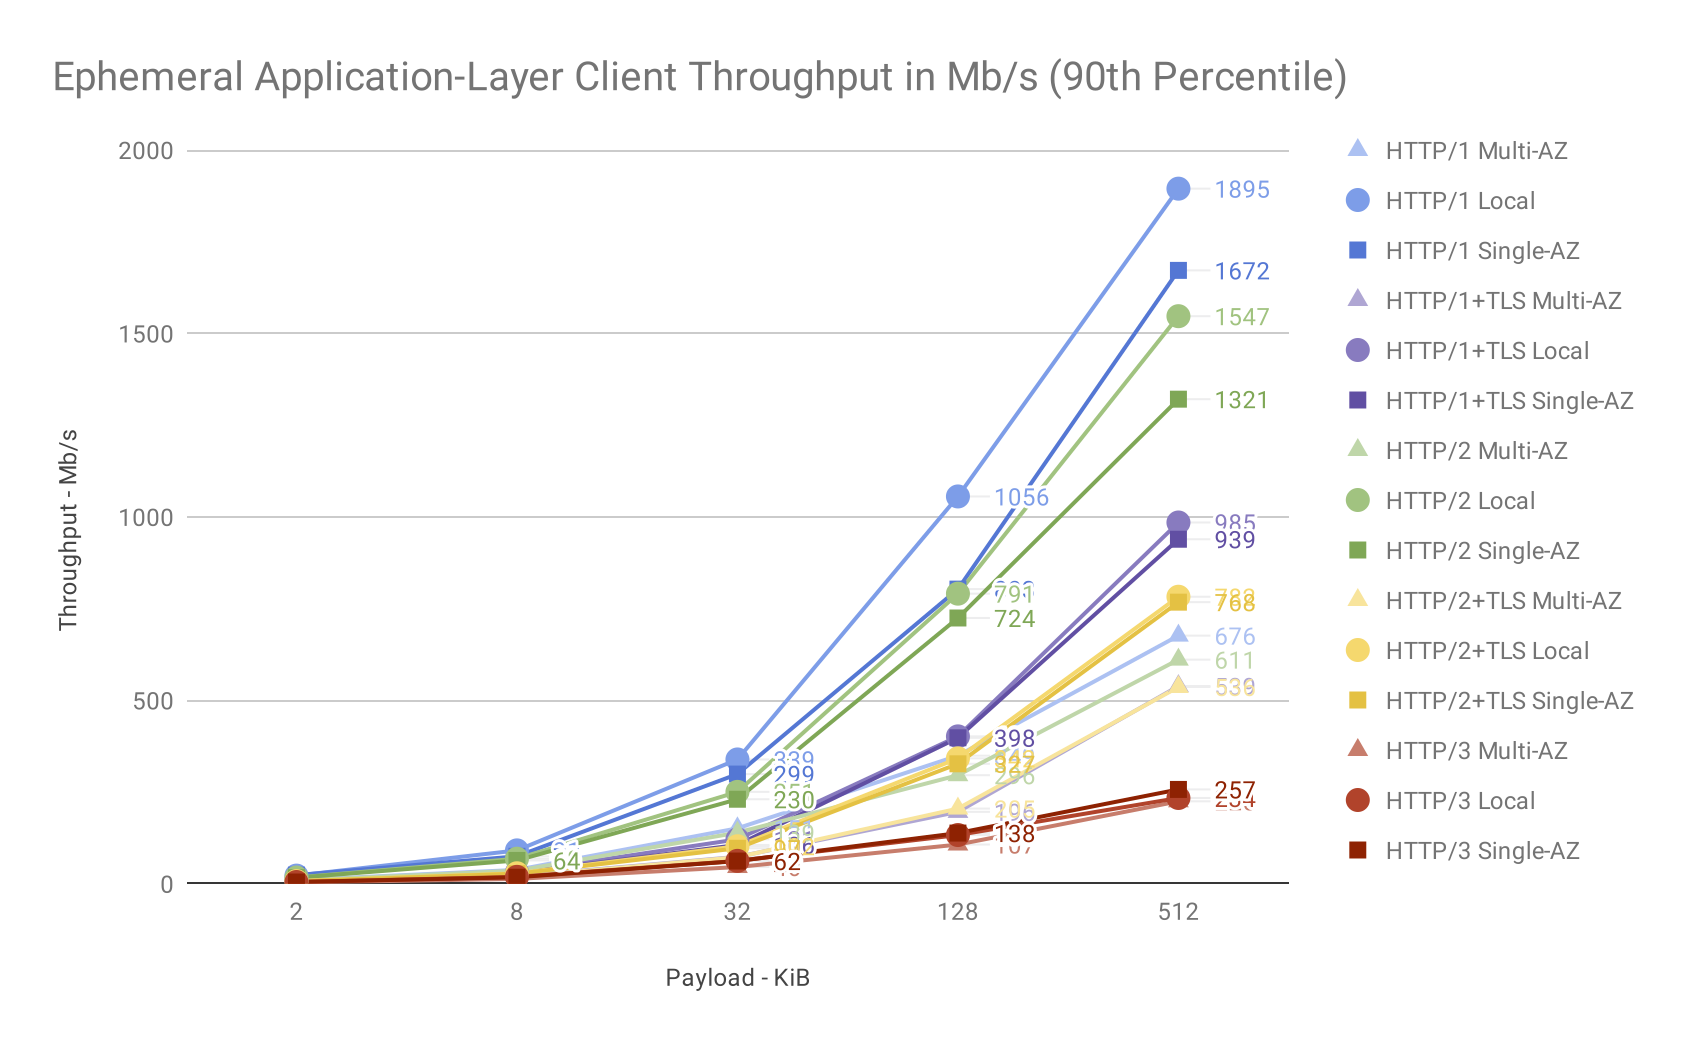
\includegraphics[width=\linewidth]{figures/charts/Ephemeral Application-Layer Client Throughput in Mb_s (90th Percentile).png}
    \caption{Ephemeral Application-Layer Client Throughput in Mb/s (90th Percentile)}
    \label{fig:ephemeral_app_throughput}
\end{figure}

\clearpage
